\documentclass[10pt]{article}
\usepackage{icmlko}

\icmlmeta{IP 파운데이션 월드모델}{98}{다섯을 쌓아도 하나만큼이다}{서로 다른 축 다섯을 쌓아도 팝업의 이득은 $+$0.022에서 멈추고, 그 천장을 설명하려던 가설은 개입 검정에서 죽었다}

\begin{document}

\twocolumn[
\icmlheader

\begin{abstract}
노트 96은 설명문 축이 팝업을 $+$0.0222 올린다고 했고, 노트 97은 표지 축이 같은
$+$0.0220을 준다고 했다. 둘은 픽셀과 글자로, 아무 관계가 없는 데이터다.
\textbf{그러면 합치면 $+$0.044여야 한다. $+$0.0161이다.} 축을 계속 쌓아 봤다 ---
설명문 c0 · 표지 · 문장 수 · 설명문 c1 · c2 다섯을 얹으면 낱개 이득의 합은
$+$0.0507인데 \textbf{실제는 $+$0.0189}이고, 그 사이 어느 조합에서도 팝업은
\textbf{$+$0.022를 못 넘는다}. 판정치는 반대로 단조로 무너진다($+$0.4142
$\to+$0.3453, 축 하나당 약 $-$0.017). \textbf{출처 쪽에 축을 더하는 길에는
천장이 있다} --- 노트 96이 ``출처 96개면 라벨 천장에 닿는다''고 셈한 것은
기울기가 계속 간다고 본 것이라 \textbf{낙관적 상한으로 낮춘다.} 천장이 왜
있는지 두 가설을 세웠다. ① \textbf{시각 경로}(노트 97의 해석) --- 팝업의
매장 노출 슬롯을 끄면 이득의 \textbf{94\%가 사라지고}(남은 6\%) 입장료를 끄면
83\%가 남는다. \textbf{살아남았다.} ② \textbf{슬롯 완전성} --- 팝업만 다섯
슬롯이 전부 100\%이고, 안 받는 네 대상의 평균 덮개율과 최선 이득의 상관이
\textbf{$r=+$0.938}이다. 그럴듯해서 개입으로 검정했다 --- 팝업의 슬롯을 무작위로
갉아 덮개율을 100\%에서 90\%로 낮췄다. \textbf{이득이 안 준다}($r=-$0.505).
\textbf{네 점의 상관은 아무것도 아니었다.}
\end{abstract}
]

\begin{figure*}[t]
\centering
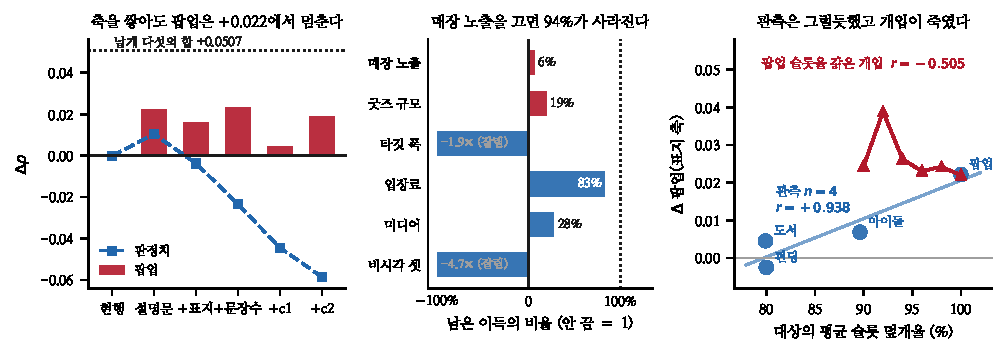
\includegraphics[width=\textwidth]{figs/sc.pdf}
\caption{왼쪽 --- 쌓아도 안 올라간다. 가운데 --- 시각 경로는 살아남는다.
오른쪽 --- 관측은 그럴듯했고 개입이 죽였다.}
\end{figure*}

\section{둘을 합치면 반도 안 된다}

\begin{table}[t]
\centering\tsize
\caption{설명문 축(여섯 도메인)과 표지 축(다섯 도메인).}
\begin{tabular}{lrrrr}
\toprule
& $\rho$ & $\Delta$ & 팝업 & $\Delta$팝업 \\
\midrule
현행 & $+$0.4038 & --- & $+$0.4501 & --- \\
설명문만 & $+$0.4142 & $+$0.0104 & $+$0.4723 & $+$0.0222 \\
표지만 & $+$0.3925 & $-$0.0113 & $+$0.4721 & $+$0.0220 \\
\textbf{둘 다} & $+$0.4000 & $-$0.0038 & $+$0.4662 & \textbf{$+$0.0161} \\
\midrule
독립이면 & & $-$0.0010 & & \textbf{$+$0.0441} \\
\bottomrule
\end{tabular}
\end{table}

픽셀에서 뽑은 축과 글자에서 뽑은 축이 팝업에 주는 것의 \textbf{63\%가 겹친다.}
내용이 겹칠 수가 없는데 겹친다.

\section{다섯을 쌓아도 하나만큼이다}

\begin{table}[t]
\centering\tsize
\caption{축을 하나씩 얹는다. 여섯 도메인.}
\begin{tabular}{lrrr}
\toprule
쌓은 것 & 개수 & 판정치 & $\Delta$팝업 \\
\midrule
현행 & 0 & $+$0.4038 & --- \\
설명문 c0 & 1 & $+$0.4142 & \textbf{$+$0.0222} \\
$+$표지 & 2 & $+$0.4000 & $+$0.0161 \\
$+$문장 수 & 3 & $+$0.3804 & \textbf{$+$0.0233} \\
$+$설명문 c1 & 4 & $+$0.3593 & $+$0.0043 \\
$+$설명문 c2 & 5 & $+$0.3453 & $+$0.0189 \\
\midrule
\multicolumn{2}{l}{낱개 다섯의 합} & & \textbf{$+$0.0507} \\
\bottomrule
\end{tabular}
\end{table}

낱개 이득은 설명문 c0 $+$0.0222 · 표지 $+$0.0220 · 문장 수 $-$0.0020 ·
설명문 c1 $+$0.0098 · c2 $-$0.0012이다.

\claimx{출처 쪽에 축을 더하는 길에 \textbf{천장이 있다.} 다섯을 쌓아도 팝업은
$+$0.022를 못 넘고, 낱개 합($+$0.0507)의 37\%만 남는다. 그러는 사이 판정치는
축 하나당 약 $-$0.017씩 단조로 무너진다.}{다섯 축을 \emph{쌓는} 실험이지
\emph{출처를 늘리는} 실험이 아니다. 노트 96의 기울기는 출처 수에 대한 것이므로
직접 반박은 아니다.}

\begin{quote}\fontsize{9.5}{11.5}\selectfont
\textbf{노트 96의 셈을 낮춘다.} 노트 96은 ``순 기울기 $+$0.0030으로 남은
0.284를 메우려면 출처 96개''라고 적었다. 그 셈은 기울기가 계속 간다고 본
것인데, 여기서 \emph{다른 방향}으로 정보를 더할 때 $+$0.022에서 멈추는 것을
봤다. \textbf{96개는 예측이 아니라 낙관적 상한이다.}
\end{quote}

\section{가설 ① 시각 경로 --- 살아남았다}

노트 97은 ``표지 축이 팝업의 매장 노출 · 굿즈 규모 슬롯과 맞는다''고 해석했다.
그 슬롯을 끄고 이득이 남는지 봤다. 시각이 아닌 슬롯을 끄는 \textbf{가짜약 팔}을
같이 뒀다.

\begin{table}[t]
\centering\tsize
\caption{팝업의 슬롯을 끄고 표지 축의 이득이 남는가.}
\begin{tabular}{lrrr}
\toprule
끈 슬롯 & 바탕 & 이득 & 남은 비율 \\
\midrule
(안 끔) & $+$0.4501 & $+$0.0220 & 100\% \\
\midrule
\textbf{매장 노출}(시각) & $+$0.4117 & $+$0.0014 & \textbf{6\%} \\
굿즈 규모(시각) & $+$0.3231 & $+$0.0042 & 19\% \\
둘 다(시각) & \multicolumn{3}{l}{팝업이 정렬 불가} \\
\midrule
입장료(가짜약) & $+$0.4177 & $+$0.0181 & \textbf{83\%} \\
미디어(가짜약) & $+$0.4467 & $+$0.0061 & 28\% \\
타깃 폭(가짜약) & $+$0.2060 & $-$0.0415 & $-$189\% \\
\bottomrule
\end{tabular}
\end{table}

\claimx{시각 경로가 살아남았다. 매장 노출을 끄면 이득의 \textbf{94\%가
사라지고}, 입장료를 끄면 83\%가 남는다. 표지의 이득은 팝업의 \emph{보이는}
슬롯을 통해 온다.}{깨끗한 대비는 매장 노출 대 입장료 둘뿐이다. 다른 시각 슬롯
(굿즈 규모)도 19\%밖에 안 남기고, 시각이 아닌 미디어도 28\%밖에 안 남긴다.
\textbf{슬롯을 끄면 팝업의 인자 공간 자체가 얇아지므로} 어느 슬롯을 꺼도 이득이
줄어드는 것이 자연스럽다 --- 가짜약이 완전한 가짜약이 아니다.}

\section{가설 ② 슬롯 완전성 --- 개입이 죽였다}

\begin{table}[t]
\centering\tsize
\caption{축을 안 받는 네 대상. 팝업만 다섯 슬롯이 전부 100\%다.}
\begin{tabular}{lrrrr}
\toprule
& $n$ & 슬롯 100\% & 평균 덮개율 & 최선 이득 \\
\midrule
\textbf{팝업} & 75 & \textbf{5} & \textbf{100\%} & \textbf{$+$0.0222} \\
아이돌 & 81 & 0 & 90\% & $+$0.0069 \\
도서 & 243 & 3 & 80\% & $+$0.0046 \\
펀딩 & 400 & 4 & 80\% & $-$0.0024 \\
\midrule
\multicolumn{3}{l}{덮개율과 이득의 상관} & & \textbf{$r=+$0.938} \\
\bottomrule
\end{tabular}
\end{table}

$r=+$0.938은 그럴듯하다. 정렬은 슬롯을 통해 이뤄지므로, 슬롯이 다 있는 대상만
출처의 새 축을 온전히 받는다는 이야기가 된다. \textbf{개입으로 검정했다} ---
팝업의 다섯 슬롯을 무작위로 갉아 덮개율을 낮추고 이득을 다시 잰다.

\begin{table}[t]
\centering\tsize
\caption{팝업 슬롯을 갉는다. 씨앗 다섯 평균.}
\begin{tabular}{lrrrr}
\toprule
덮개율 & 완전 사례 & 바탕 & 표지 이득 & 설명문 이득 \\
\midrule
100\% & 75 & $+$0.4501 & $+$0.0220 & $+$0.0222 \\
98\% & 69 & $+$0.4581 & $+$0.0242 & $+$0.0231 \\
96\% & 60 & $+$0.4296 & $+$0.0230 & $+$0.0274 \\
94\% & 53 & $+$0.4402 & $+$0.0263 & $+$0.0282 \\
92\% & 47 & $+$0.4514 & \textbf{$+$0.0388} & \textbf{$+$0.0350} \\
90\% & 42 & $+$0.4515 & $+$0.0243 & $+$0.0168 \\
\midrule
\multicolumn{3}{l}{덮개율과의 상관} & \textbf{$-$0.505} & $-$0.080 \\
\bottomrule
\end{tabular}
\end{table}

\claimx{슬롯 완전성 가설은 \textbf{틀렸다.} 팝업의 덮개율을 100\%에서 90\%로
낮춰도 이득이 안 줄고 오히려 는다($r=-$0.505). \textbf{네 점의 관측 상관
$+$0.938은 아무것도 아니었다.}}{개입 쪽도 깨끗하지 않다 --- 덮개율을 갉으면
완전 사례가 75건에서 42건으로 준다(\texttt{factor\_space} 가 완전 사례만 쓴다,
노트 84). 표본이 작아지면 순위 상관 자체가 흔들린다. \textbf{덮개율을 80\%까지
낮추면 바탕이 $+$0.5547로 뛰어 못 견주므로 90\% 위에서만 읽었다.}}

이 프로젝트에서 관측 상관이 개입에 죽은 것이 처음은 아니다 --- 노트 67(작은
표본 배선) · 80(부분집합) · 82(분모) · 91$\to$92(성분 수)에 이어 다섯 번째다.
\textbf{다만 이번은 $r=+$0.938로 가장 그럴듯했다.}

\section{그래서 천장은 왜 있나}

모른다. 남은 것은 이렇다.

\begin{itemize}[leftmargin=1.1em,itemsep=0.15em]
\item 살아남은 것 --- \textbf{시각 경로}(매장 노출을 끄면 94\% 사라짐).
      단, 어느 슬롯을 꺼도 얼마씩은 준다.
\item 죽은 것 --- \textbf{슬롯 완전성}($r=+$0.938 관측, 개입 $-$0.505).
\item 죽은 것 --- \textbf{덧셈}(픽셀 축과 글자 축이 63\% 겹친다).
\item 안 본 것 --- 출처 \emph{수}를 6개 너머로 늘렸을 때도 멈추는가. 이것이
      노트 96의 셈을 진짜로 판정한다.
\end{itemize}

\section{한계}

\begin{itemize}[leftmargin=1.1em,itemsep=0.15em]
\item 이 노트의 어느 설정도 \textbf{채택하지 않는다.} 표지 축은 판정치 악화
      4/4(노트 97)이고 쌓기는 판정치를 $-$0.058까지 깎는다.
\item 팝업 이득의 붓스트랩 구간이 $[-0.032, +0.074]$로 넓다($n{=}75$).
      $+$0.0161과 $+$0.0233을 가를 수 없다.
\item 슬롯 끄기의 가짜약 팔이 완전한 가짜약이 아니다 --- 어느 슬롯을 꺼도
      인자 공간이 얇아진다.
\item 갉기 개입이 표본 크기와 얽혀 있다. 덮개율만 따로 못 움직였다.
\item ``천장 $+$0.022''는 다섯 축 · 여섯 도메인에서의 관측이다. 다른 축
      종류로는 넘을 수 있다.
\end{itemize}

\section{다음}

\begin{enumerate}[leftmargin=1.3em,itemsep=0.15em]
\item \textbf{출처 수를 늘려 천장을 친다} --- 노트 96의 셈을 판정하는 유일한
      길이다. 설명문 있는 도메인을 여섯에서 여덟 · 열로 늘리고 곡선이 휘는지
      본다. 새 도메인이 필요하다.
\item \textbf{대상 쪽을 늘린다} --- 팝업 · 아이돌 · 도서 · 펀딩에 설명문 ·
      표지를 붙인다. 지금까지 전부 출처 쪽 이야기였고, 대상이 좋아지는 길은
      한 번도 안 열었다.
\item 시각 경로를 제대로 가른다 --- 슬롯을 끄는 대신 \textbf{뒤섞어서}
      인자 공간의 두께를 유지한 채 대응만 깬다(노트 53의 규약).
\item 팝업 표본. $[-0.032, +0.074]$가 모든 결론을 흐린다(노트 92).
\end{enumerate}

\vspace{0.6em}
\hrule height 0.3pt
\vspace{0.5em}
{\footnotesize
\textbf{참고문헌}\\[0.3em]
Pearl, J. (2009). \emph{Causality: Models, Reasoning, and Inference}, 2nd ed.
Cambridge University Press.\\[0.15em]
Schoenemann, P. H. (1966). A generalized solution of the orthogonal Procrustes
problem. \emph{Psychometrika}, 31(1), 1--10.\\[0.15em]
Little, R. J. A., Rubin, D. B. (2019). \emph{Statistical Analysis with Missing
Data}, 3rd ed. Wiley.\\[0.15em]
Simpson, E. H. (1951). The interpretation of interaction in contingency tables.
\emph{JRSS B}, 13(2), 238--241.\\[0.15em]
Efron, B., Tibshirani, R. J. (1993). \emph{An Introduction to the Bootstrap}.
Chapman \& Hall.
}

\end{document}
